\section{Proposta experimental}



%%%%%%%%%%%%%%%%%%%%%%%%%%%%%%%%%%%%%%%%%%%%%%%%%%%%%%%%%%%%%%%%%%%%%%%%%%%%%%%%

%%%%%%%%%%%%%%%%%%%%%%%%%%%%%%%%%%%%%%%%%%%%%%%%%%%%%%%%%%%%%%%%%%%%%%%%%%%%%%%%
\begin{frame}
\frametitle{Criação da base de dados}

\begin{itemize}
\item Pessoas no experimento: 40 pessoas.
\item Quantidade de imagens: 40 mil - 60 mil.
\item Quantidade de avaliadores: 3 profissões da área da saúde.
\item Local do experiemtno: Hospital.
\end{itemize}


\end{frame}

%%%%%%%%%%%%%%%%%%%%%%%%%%%%%%%%%%%%%%%%%%%%%%%%%%%%%%%%%%%%%%%%%%%%%%%%%%%%%%%%

\begin{frame}
\frametitle{Coleta de informação: manequim }
\begin{figure}[!ht]
    \centering
    \caption{Base de dados .}
    \begin{minipage}[t]{0.55\textwidth}
    \centering
      \includegraphics[width=0.95\textwidth]{images/2022-08-22 12-53-22.png}
      \subcaption{Manequim para a simulação artificial do paciente (Fonte: Sitio web \url{https://www.unoeste.br/lhabsim/Content/documentos/Lista-Equipamentos.pdf}). \label{fig:2022-08-22 12-53-22}}
    \end{minipage}
    \hfill
    \begin{minipage}[t]{0.35\textwidth}
    \centering
      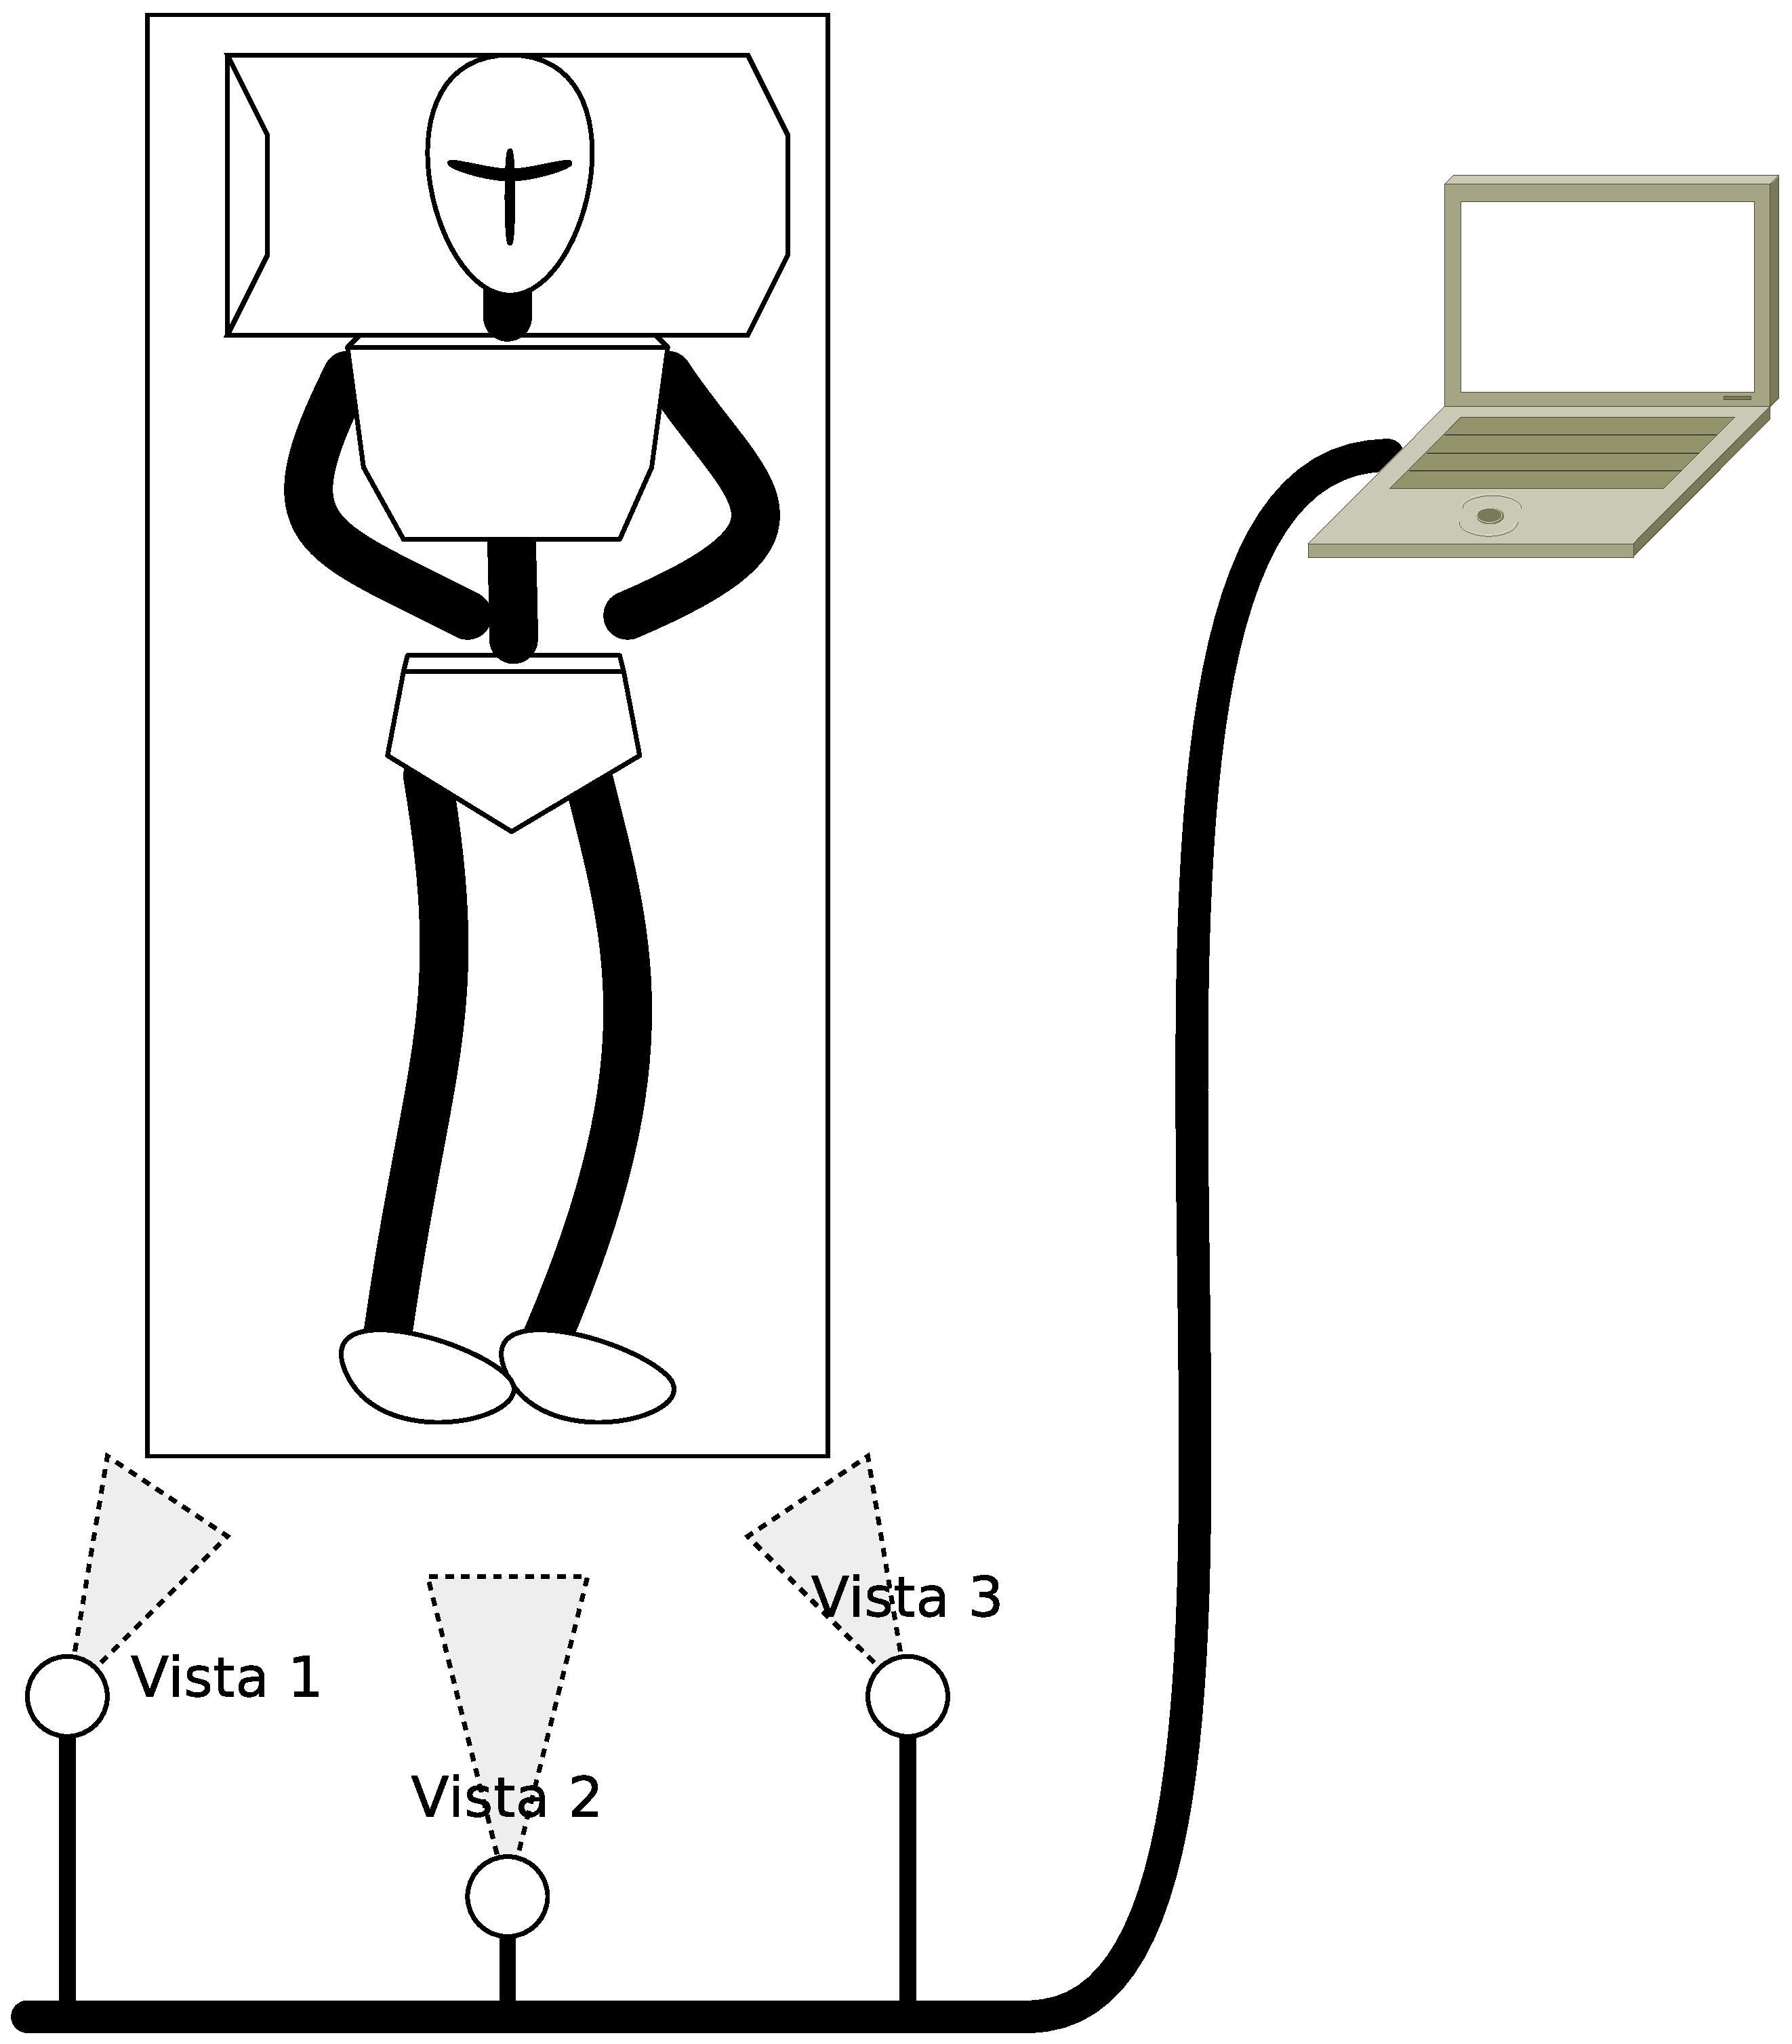
\includegraphics[width=0.95\textwidth]{images/multiview.eps}
      \subcaption{Multiplas vistas (Fonte: Autor). \label{fig:multiview:3}}
    \end{minipage}
    \label{fig:manequim}
  \end{figure}
\end{frame}




%%%%%%%%%%%%%%%%%%%%%%%%%%%%%%%%%%%%%%%%%%%%%%%%%%%%%%%%%%%%%%%%%%%%%%%%%%%%%%%%
\begin{frame}
    \frametitle{Base de dados com dados dos pacientes }
    \begin{figure}[!ht]
        \centering
        \caption{Base de dados (Fonte: DALL-E).}
        \begin{minipage}[t]{0.23\textwidth}
        \centering
          \includegraphics[width=0.95\textwidth]{images/happy/DALL·E 2022-09-13 17.02.06 - full body patient in bed with a happy face.png}
          \subcaption{Positivo \label{fig:Emotion:a}}
        \end{minipage}
        \hfill
        \begin{minipage}[t]{0.23\textwidth}
        \centering
          \includegraphics[width=0.95\textwidth]{images/neutral/DALL·E 2022-09-13 17.00.22 - full body patient in bed with an emotionless face.png}
          \subcaption{Neutro \label{fig:Emotion:b}}
        \end{minipage}
        \hfill
        \begin{minipage}[t]{0.23\textwidth}
        \centering
          \includegraphics[width=0.95\textwidth]{images/depression/DALL·E 2022-09-13 17.11.39 - full body patient in bed with depression.png}
          \subcaption{Negativo \label{fig:Emotion:c}}
        \end{minipage}
        \hfill
        \begin{minipage}[t]{0.23\textwidth}
        \centering
          \includegraphics[width=0.95\textwidth]{images/pain/DALL·E 2022-09-13 17.06.15 - full body patient in bed with a pain face.png}
          \subcaption{Dor \label{fig:Emotion:d}}
        \end{minipage}
        \label{fig:patient:emotion}
      \end{figure}
    \end{frame}

%%%%%%%%%%%%%%%%%%%%%%%%%%%%%%%%%%%%%%%%%%%%%%%%%%%%%%%%%%%%%%%%%%%%%%%%%%%%%%%%

\section{Outras bases de dados}

%%%%%%%%%%%%%%%%%%%%%%%%%%%%%%%%%%%%%%%%%%%%%%%%%%%%%%%%%%%%%%%%%%%%%%%%%%%%%%%%

\begin{frame}
\frametitle{\textbf{FER2013}}
%%https://paperswithcode.com/paper/facial-expression-recognition-using-residual
\textbf{FER2013}: 23 mil imagens de 48x48 pixel.
Etiquetadas com 7 categorias:
ira, desgosto, medo, felicidade, tristeza, surpresa, neutro.
\begin{figure}[!ht]
    \centering
    \caption{Base de dados FER2013.}
    \begin{minipage}[t]{0.20\textwidth}
    \centering
      \includegraphics[width=0.75\textwidth]{images/fer2013/angry.jpg}
      \subcaption{Bravo \label{angry}}
    \end{minipage}
    \hfill
    \begin{minipage}[t]{0.20\textwidth}
    \centering
      \includegraphics[width=0.75\textwidth]{images/fer2013/disgust.jpg}
      \subcaption{Desgosto \label{disgust}}
    \end{minipage}
    \hfill
    \begin{minipage}[t]{0.20\textwidth}
    \centering
      \includegraphics[width=0.75\textwidth]{images/fer2013/fear.jpg}
      \subcaption{Medo \label{fear}}
    \end{minipage}
    \hfill
    \begin{minipage}[t]{0.20\textwidth}
    \centering
      \includegraphics[width=0.75\textwidth]{images/fer2013/happy.jpg}
      \subcaption{Feliz \label{happy}}
    \end{minipage}
    \hfill
    \begin{minipage}[t]{0.20\textwidth}
    \centering
      \includegraphics[width=0.75\textwidth]{images/fer2013/neutral.jpg}
      \subcaption{Neutral \label{neutral}}
    \end{minipage}
    \hfill
    \begin{minipage}[t]{0.20\textwidth}
    \centering
      \includegraphics[width=0.75\textwidth]{images/fer2013/sad.jpg}
      \subcaption{Triste \label{sad}}
    \end{minipage}
    \hfill
    \begin{minipage}[t]{0.20\textwidth}
    \centering
      \includegraphics[width=0.75\textwidth]{images/fer2013/surprise.jpg}
      \subcaption{Surpresa \label{surprise}}
    \end{minipage}
    \label{fig:fer2013}
  \end{figure}
\end{frame}

%%%%%%%%%%%%%%%%%%%%%%%%%%%%%%%%%%%%%%%%%%%%%%%%%%%%%%%%%%%%%%%%%%%%%%%%%%%%%%%%

\begin{frame}
\frametitle{\textbf{FER2013} - Validação cruzada}
\begin{figure}[!ht]
    \centering
    \caption{Face - Emotion - FER2013}
    \includegraphics[width=0.98\textwidth]{images/face_emotion_fer2013/crossval.png}
\end{figure}
\end{frame}

%%%%%%%%%%%%%%%%%%%%%%%%%%%%%%%%%%%%%%%%%%%%%%%%%%%%%%%%%%%%%%%%%%%%%%%%%%%%%%%%

\begin{frame}
\frametitle{\textbf{FER2013} - Testing}
\begin{figure}[!ht]
    \centering
    \caption{Face - Emotion - FER2013}
    \includegraphics[width=0.98\textwidth]{images/face_emotion_fer2013/testing.png}
\end{figure}
\end{frame}


%%%%%%%%%%%%%%%%%%%%%%%%%%%%%%%%%%%%%%%%%%%%%%%%%%%%%%%%%%%%%%%%%%%%%%%%%%%%%%%%

\begin{frame}
\frametitle{\textbf{Patient - people}}
631 imagens para treinamento e 273 para teste
\begin{figure}[!ht]
    \centering
    \caption{Patient - people}
    \includegraphics[width=0.6\textwidth]{images/cnn_patient_people/0-info.png}
\end{figure}
\end{frame}

%%%%%%%%%%%%%%%%%%%%%%%%%%%%%%%%%%%%%%%%%%%%%%%%%%%%%%%%%%%%%%%%%%%%%%%%%%%%%%%%

\begin{frame}
\frametitle{\textbf{Patient - people}}
\begin{figure}[!ht]
    \centering
    \caption{Validação cruzada - Patient - people}
    \includegraphics[width=0.9\textwidth]{images/cnn_patient_people/crossval.png}
\end{figure}
\end{frame}

%%%%%%%%%%%%%%%%%%%%%%%%%%%%%%%%%%%%%%%%%%%%%%%%%%%%%%%%%%%%%%%%%%%%%%%%%%%%%%%%

\begin{frame}
\frametitle{\textbf{Patient - people}}
\begin{figure}[!ht]
    \centering
    \caption{Testing - Patient - people}
    \includegraphics[width=0.9\textwidth]{images/cnn_patient_people/testing.png}
\end{figure}
\end{frame}

%%%%%%%%%%%%%%%%%%%%%%%%%%%%%%%%%%%%%%%%%%%%%%%%%%%%%%%%%%%%%%%%%%%%%%%%%%%%%%%%

\begin{frame}
\frametitle{4 emoções - \textbf{Patient - people}}
631 imagens para treinamento e 273 para teste
\begin{figure}[!ht]
    \centering
    \caption{4 emoções - Patient - people}
    \includegraphics[width=0.6\textwidth]{images/cnn_patient_people/0-info.png}
\end{figure}
\end{frame}

%%%%%%%%%%%%%%%%%%%%%%%%%%%%%%%%%%%%%%%%%%%%%%%%%%%%%%%%%%%%%%%%%%%%%%%%%%%%%%%%

\begin{frame}
\frametitle{4 emoções - \textbf{Patient - people}}
\begin{figure}[!ht]
    \centering
    \caption{4 emoções - Patient - people}
    \includegraphics[width=0.9\textwidth]{images/cnn_emotion4_patient_people/crossval.png}
\end{figure}
\end{frame}
%%%%%%%%%%%%%%%%%%%%%%%%%%%%%%%%%%%%%%%%%%%%%%%%%%%%%%%%%%%%%%%%%%%%%%%%%%%%%%%%

\begin{frame}
\frametitle{4 emoções - \textbf{9 pessoas}}
4800 images por pessoa, 9 pessoas 
\begin{figure}[!ht]
    \centering
    %\caption{Base de dados FER2013.}
    \begin{minipage}[t]{0.45\textwidth}
    \centering
      \includegraphics[width=0.75\textwidth]{images/new/frame_count10_cam2.png}
      %\subcaption{Bravo \label{angry}}
    \end{minipage}
    \hfill
    \begin{minipage}[t]{0.45\textwidth}
    \centering
      \includegraphics[width=0.75\textwidth]{images/new/frame_count17_cam2.png}
      %\subcaption{Desgosto \label{disgust}}
    \end{minipage}
    \hfill
    \begin{minipage}[t]{0.45\textwidth}
    \centering
      \includegraphics[width=0.75\textwidth]{images/new/frame_count41_cam1.png}
      %\subcaption{Medo \label{fear}}
    \end{minipage}
    \hfill
    \begin{minipage}[t]{0.45\textwidth}
    \centering
      \includegraphics[width=0.75\textwidth]{images/new/frame_count26_cam1.png}
      %\subcaption{Feliz \label{happy}}
    \end{minipage}
    \label{fig:fer2013}
  \end{figure}
\end{frame}
\end{frame}
%%%%%%%%%%%%%%%%%%%%%%%%%%%%%%%%%%%%%%%%%%%%%%%%%%%%%%%%%%%%%%%%%%%%%%%%%%%%%%%%

\begin{frame}
\frametitle{Fim}

{ \Huge Obrigado!}

\end{frame}

